Vier gleiche, homogene Bretter sind je um eine waagrechte, reibungsfreie Achse durch den Punkt D drehbar. S ist jeweils der Schwerpunkt des Bretts. Die Achse liegt
\begin{itemize}
 \item bei Brett 1 \SI{10}{\cm} senkrecht über S,
 \item bei Brett 2 \SI{10}{\cm} senkrecht unter S,
 \item bei Brett 3 genau in S,
 \item bei Brett 4 \SI{10}{\cm} rechts von S, auf gleicher Höhe.
\end{itemize}
Jedes Brett wird in der gezeichneten Lage aus der Ruhe losgelassen.
\begin{center}
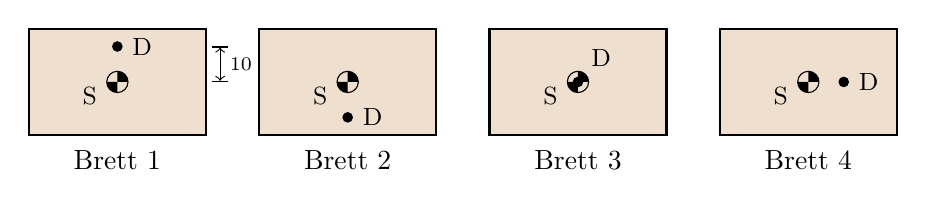
\begin{tikzpicture}[scale=0.45]
 \foreach \x/\dx/\dy/\n in {0/0/1/1, 6.5/0/-1/2, 13/0/0/3, 19.5/1/0/4} {
  \begin{scope}[shift={(\x,0)}]
   \fill[brown!25] (-2.5,-1.5) rectangle (2.5,1.5);
   \draw[thick] (-2.5,-1.5) rectangle (2.5,1.5);
   \draw (0,0) circle (0.3); \fill (0,0) -- (0.3,0) arc (0:90:0.3) -- cycle; \fill (0,0) -- (-0.3,0) arc (180:270:0.3) -- cycle;
   \fill (\dx,\dy) circle (0.15);
   \node at (0,-2.2) {Brett \n};
  \end{scope}
 }
 \node[left] at (-0.3,-0.4) {\small S}; \node[right] at (0.15,1) {\small D};
 \node[left] at (6.2,-0.4) {\small S}; \node[right] at (6.65,-1) {\small D};
 \node[left] at (12.7,-0.4) {\small S}; \node[above right] at (13.1,0.15) {\small D};
 \node[left] at (19.2,-0.4) {\small S}; \node[right] at (20.65,0) {\small D};
 \draw[|<->|] (2.9,0) -- (2.9,1) node[midway, right] {\scriptsize \SI{10}{\cm}};
\end{tikzpicture}
\end{center}

\begin{abcliste}
\abc
Ist das Brett jeweils im Gleichgewicht? Wenn ja: Ist das Gleichgewicht stabil, labil oder indifferent? \DuSie{Begründe}{Begründen Sie} mit dem Drehmoment der Gewichtskraft bezüglich D.

\abc
Was geschieht mit Brett 4? In welcher Lage käme es zur Ruhe, wenn die Achse doch ein wenig Reibung hätte?
\end{abcliste}
